\documentclass[10pt]{beamer}

\usetheme[progressbar=frametitle]{metropolis}
\usepackage{appendixnumberbeamer}

\usepackage{booktabs}
\usepackage[scale=2]{ccicons}

\usepackage{pgfplots}
\usepgfplotslibrary{dateplot}

\usepackage{xspace}
\newcommand{\themename}{\textbf{\textsc{metropolis}}\xspace}

\usepackage[english]{babel}
\usepackage{tikz}
\usepackage{pgfplots}
\usepackage{caption}
\usepackage{circuitikz}
\usepackage{listings}
\usepackage{pgfplotsthemetol}
\captionsetup{justification=centering}
\usetikzlibrary{plotmarks}
\usepackage[utf8]{inputenc}
\usepackage[english]{babel}
\usepackage{amsmath}
\usepackage{amsfonts}
\usepackage{amssymb}
\usepackage{graphicx}
\usepackage{setspace}
\usepackage{parskip}
\usepackage{amsthm}
\usepackage{fancyhdr}
\usepackage{booktabs}
\usepackage{hyperref}
\usepackage{pgfplots}% This uses tikz
\pgfplotsset{compat=newest}% use newest version
\usepackage{sidecap}
\usepackage{tikz}
\usepackage{tikz-3dplot}
\usepackage{xcolor}
\usepackage{xstring}
\usepackage{multirow}
\usepackage{adjustbox}

\usepackage{caption}
\usepackage{color}
\usepackage{array}
\usepackage{wrapfig}
\usepackage{listings}

\captionsetup{justification=centering}
\usetikzlibrary{plotmarks}

\usepackage{lipsum}% http://ctan.org/pkg/lipsum
\usepackage{hanging}% http://ctan.org/pkg/hanging
\setbeamertemplate{footnote}{%
  \hangpara{2em}{1}%
  \makebox[2em][l]{\insertfootnotemark}\footnotesize\insertfootnotetext\par%
}


\usepackage[scale=2]{ccicons}
\usepackage{minted}

\usemintedstyle{trac}
\definecolor{mDarkTeal}{HTML}{23373b}
\setbeamercolor{section page}{bg=mDarkTeal}

%*******************************************************************************

\title{SCELP: Low Delay Audio Coding with Noise Shaping Based on Spherical Vector Quantization}
\subtitle{Coding of Audiovisual Contents}
\date{Barcelona, \today}
\author{Miquel Oller Oliveras \& Alvaro Scherk Fontanals}
\institute{ \vspace{40pt} \includegraphics[height=20pt]{./img/logoUPC.png}\hspace{75pt}
\includegraphics[height=20pt]{./img/etsetb3.png}}

%*******************************************************************************
\begin{document}

\maketitle

\begin{frame}{Table of Contents:}
  \tableofcontents
\end{frame}


% SECTION 1: ======================================================================

\begingroup
\setbeamercolor{section title}{fg=white}
\setbeamercolor{background canvas}{bg=mDarkTeal}
\section{SCELP}
\endgroup


% SLIDE 1: _____________________________________________________________________
\begin{frame}{Abstract}
\centering
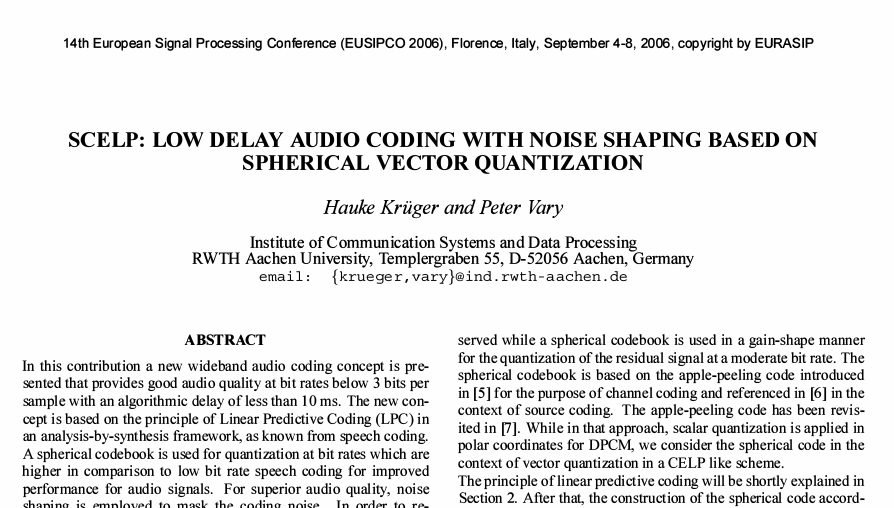
\includegraphics[width =0.7\linewidth]{./img/overview.png}
  \begin{itemize}
    \item Good audio quality at bit rates below 3 bits per sample
    \item Based in LPC with analysis-by-synthesis framework
    \item Spherical codebook for quatization
    \item Masked coding noise
    \item All-pole filter models spectral envelope of input signal
  \end{itemize}
\end{frame}
%La propuesta de los autores consiste en un nuevo sistema para obtener calidad de audio a bit rates bajos (48 kbits/s). Para ello emplean un sistema basado en el Linear prediction coding usando analysis-by-synthesis (lazo cerrado) e integrando un codebook esferico para la cuatizacion(a explicar mas adelante). adicionalmente se emplea "noise shaping" para enmascarar el ruido de codificacion. El modelo empleado es el más habitual en el mundo de las comunicaciones y usa un filtro todo-polos para modelar la envolvente espectral de la entrada, y, en funcion de este filtro, se calcula el LP resiudal a traves del inverso del filtro anterior, el cual se cuantifica.

% SLIDE 2: _____________________________________________________________________
\begin{frame}{Adaptative Linear Prediction }
\begin{itemize}
  \item Windowed segment of length $L_{lpc}$ to obtain coefficients
  \item Coefficients must be sent together with the cuantized residual LP
  \item Vector quantization instead of scalar\footnotemark
\end{itemize}
\centering
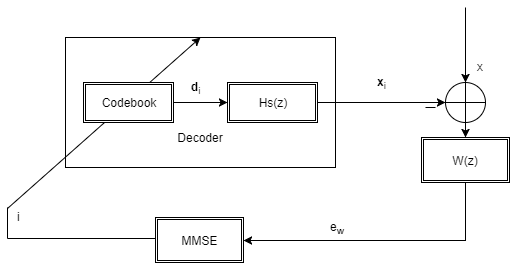
\includegraphics[width=0.8\linewidth]{./img/Figure_1.png}
\footnotetext[1]{Hola bon dia}
\end{frame}
% Al hacer prediccion lineal adapativa la señal de entrada se evalua en ventanas de longitud Llpc, a partir de dichas evalcuaciones se obitenen los coeficientes VARIANTES con los que se construye el filtro LP de ANALISIs, el cual nos da la señal residual LP. Dicha señal se cuantiza y transmite al decodificador. El filtro de SINTESIS (inverso del anterior) reconstruye la señal original (lo mejor que puede) a traves de dicho filtro en el decodificador. En el caso a tratar los coeficientes deben ser enviados junto con la señal residual cuantizada, esto supone un aumento no significante en el bit rate.

% Al usar cuantizacion vectorial (muchas nuestras de la señal LP residual se juntan en un vecttor de longitud Lv) se obtienen beneficios que no aparecen al usar la escalar. Para ello se emplea colsed loop en el lado del codificador, a través de esto se encuentra el vector cuantizado optimo  a usar como excitacion del LP residual. Explicar funcionamineto acompañado del esquema Figura 1: Analysis-by-synthesis for VQ

% SECTION 2:====================================================================

\begingroup
\setbeamercolor{section title}{fg=white}
\setbeamercolor{background canvas}{bg=mDarkTeal}
\section{Spherical Codebook}
\endgroup

% SLIDE : _____________________________________________________________________
\begin{frame}{Spherical Codebook}
  \begin{itemize}
    \item Codewords composed by:
    \begin{itemize}
      \item gain (scalar)
      \item shape (vector)
    \end{itemize}
    \item Apple-peeling rule
    \end{itemize}
  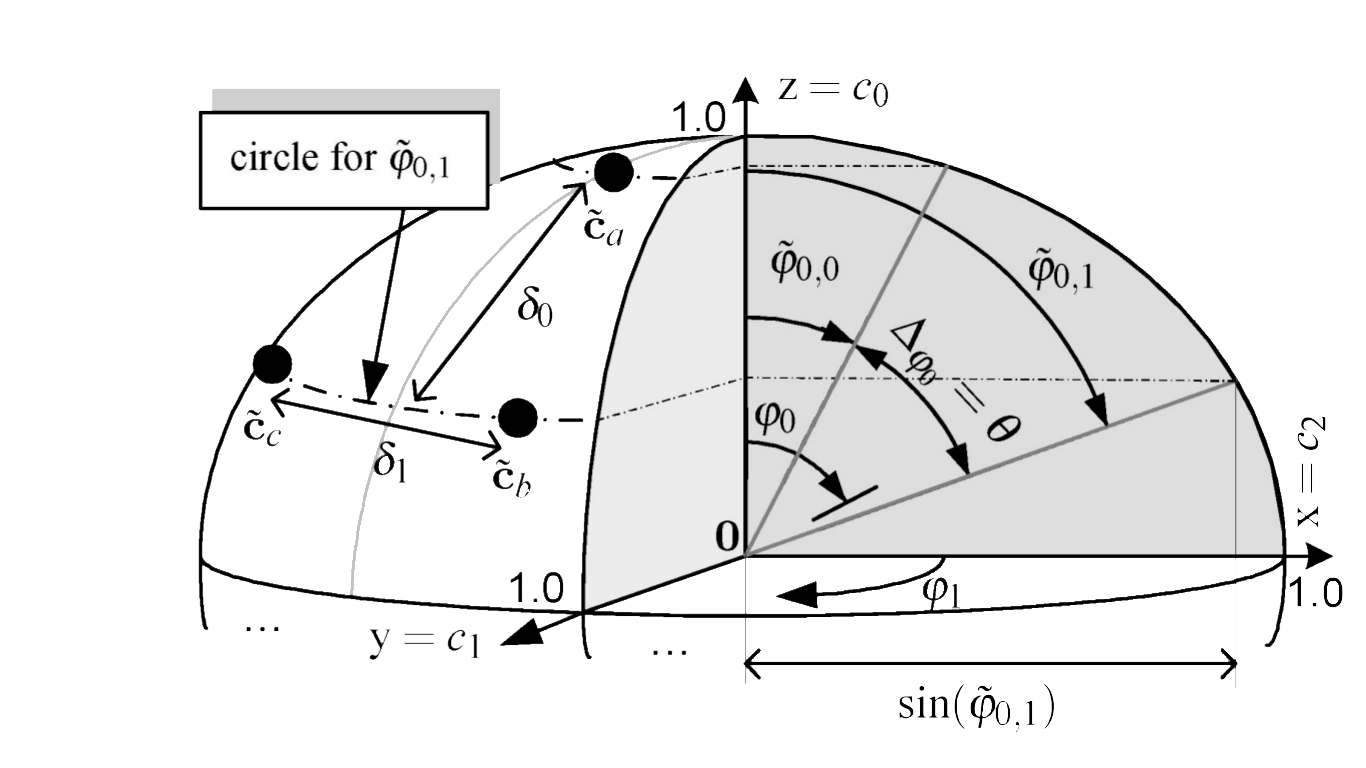
\includegraphics[width=0.9\linewidth]{./img/Centroides.png}
  \footnotemark
    % El codebook esferico tiene sus vectores compuestos por una ganancia (gain) que es un escalar y un vector llamado forma (shape). Los vectores están en el radio unidad de la esfera, y la ganancia es el radio cuantizado.
    % Se usa el metodo applepeeling para encontrar el codebook dentro del espacio Lv-dimensional. Conduicion de diseño : Llpc/Lv entero, para tener distribucion uniforme en el radio de la esfera
              %Figura 2: 3-dimensional sphere for apple-peeling code. explicarla bien.
  \footnote{Image from paper}
\end{frame}

% SLIDE : _____________________________________________________________________
\begin{frame}{Spherical Codebook Construction: 3D model}
  \begin{itemize}
    \item $\theta (Nsp) = \pi$ / Nsp where Nsp denotes the number of sublayers.
    \item Angle is given by expression (4)
    \item Separation between circles (5)
    \item Number of intervals in each circle (6)
    \item Finally, centroids are given by (7)
    % La esfera se divide en circulos separados pi/Nsp, de manera que la distancia entre circulos sera pi/Nsp, dichos circulos se encuentran en los angulos obtenidos por la expresion (4). Los centroides siguen la expresion (7), donde Nsp1 es el numero de itnervalos en cada circumferencia.
              % insertar ecuacion (4), (5), (6), (7)
  \end{itemize}
\end{frame}

% SLIDE : _____________________________________________________________________
\begin{frame}{Spherical Codebook: Cartesian Coordinates of centroids}
  \begin{itemize}
    \item Cartessian coordinates:
    \begin{equation*}
      x_{1} = r \cdot cos(\phi_{1})
    \end{equation*}
    \begin{equation*}
      x_{2} = r \cdot sin(\phi_{1}) \cdot cos(\phi_{2})
    \end{equation*}
    \begin{equation*}
      x_{3} = r \cdot sin(\phi_{1}) \cdot sin(\phi_{2}) \cdot cos(\phi_{3})
    \end{equation*}
    \centering $\vdots$
    \begin{equation*}
      x_{n-1} = r \cdot sin(\phi_{1}) \cdot \dotsc \cdot sin(\phi_{n-2}) \cdot cos(\phi_{n-1})
    \end{equation*}
    \begin{equation*}
      x_{n} = r \cdot sin(\phi_{1}) \cdot \dotsc \cdot sin(\phi_{n-2})  \cdot sin(\phi_{n-1})
    \end{equation*}
              % insertar ecuacion (8)
    % Dado que la esfera no es necesariamente tridimensional pasar de coordenadas esfericas a cartesianas no es evidente. Proceso costoso computacionalmente reducido mediante uso de tablas con los valores. para todos las dimensiones menos la última: coseno del angulo * producto de los senos de los anteriores. Para el ultimo: producto de senos anteriores
  \end{itemize}
\end{frame}

% SLIDE : _____________________________________________________________________
\begin{frame}{Spherical Codebook: N-Spherical Coordinates of Centroids}
  \begin{itemize}
    \item Sherical coordinates:
    \begin{equation*}
      r = \sqrt{x_{n}^2 + x_{n-1}^2 + \dotsc + x_{2}^2 + x_{1}^2}
    \end{equation*}
    \begin{equation*}
      \phi_{1} = arccot \frac{x_{1}}{\sqrt{x_{n}^2 + x_{n-1}^2 + \dotsc + x_{2}^2}} = arccos \frac{x_{1}}{\sqrt{x_{n}^2 + x_{n-1}^2 + \dotsc + x_{2}^2 + x_{1}^2}}
    \end{equation*}
    \begin{equation*}
      \phi_{2} = arccot \frac{x_{2}}{\sqrt{x_{n}^2 + x_{n-1}^2 + \dotsc + x_{3}^2}} = arccos \frac{x_{2}}{\sqrt{x_{n}^2 + x_{n-1}^2 + \dotsc + x_{2}^2}}
    \end{equation*}
    \centering $\vdots$
    \begin{equation*}
      \phi_{n-2} = arccot \frac{x_{n-2}}{\sqrt{x_{n}^2 + x_{n-1}^2}} = arccos \frac{x_{n-2}}{\sqrt{x_{n}^2 + x_{n-1}^2 + x_{n-2}^2}}
    \end{equation*}
    \begin{equation*}
      \phi_{n-1} = 2*arccot\frac{x_{n-1} + \sqrt{x_{n}^2 + x_{n-1}^2}}{x_{n}}
    \end{equation*}
              % insertar ecuacion (8)
    % Dado que la esfera no es necesariamente tridimensional pasar de coordenadas esfericas a cartesianas no es evidente. Proceso costoso computacionalmente reducido mediante uso de tablas con los valores. para todos las dimensiones menos la última: coseno del angulo * producto de los senos de los anteriores. Para el ultimo: producto de senos anteriores
  \end{itemize}
\end{frame}

  % SLIDE : _____________________________________________________________________
  \begin{frame}{Optimized Excitation Search}
      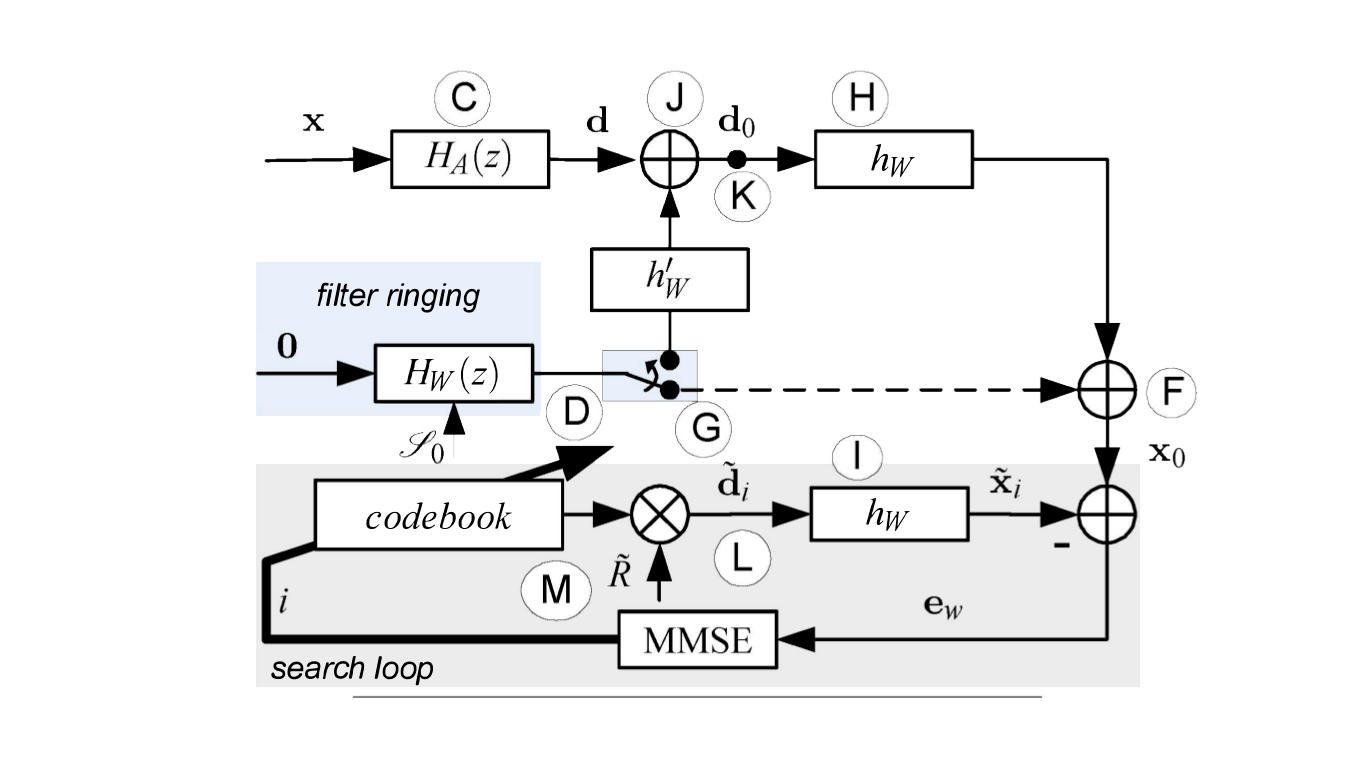
\includegraphics[width=\linewidth]{./img/closed_loop_scheme_complex.png}
              %Figure 3: modified analysis-by-synthesis

      %Dado que pueden haber muchos posibles vectores el sistema original se modifica para hacerlo más eficiente/facil de obtener, explciar el nuevo esquema. Se emplean dos tecnicas para reducir la complejidad: preselccion que reduce la complejidad y exclusiond e candidatos, que aunque añada ruido simplifica mucho la complejidad compuacional.

  \end{frame}

  % SLIDE : _____________________________________________________________________
  \begin{frame}{Preselection}
    \begin{itemize}
      \item Select neighbour centroids surrounding the unquantized signal
      \item  2 new layer candidates for each layer. Select the upper and lower circumdferences for each $\phi_i$
      \item $2^{L_v -1}$ total neighbours which are the candidates
      % Se computa la distorsion de todos los vecinos y se utiliza aquel que introduzca menos distorsion. Se puede profundizar mas en este punto, pero al ser secundario y no saber la longitud de la totalidad lo dejare asi por ahora.
    \end{itemize}
    \centering
    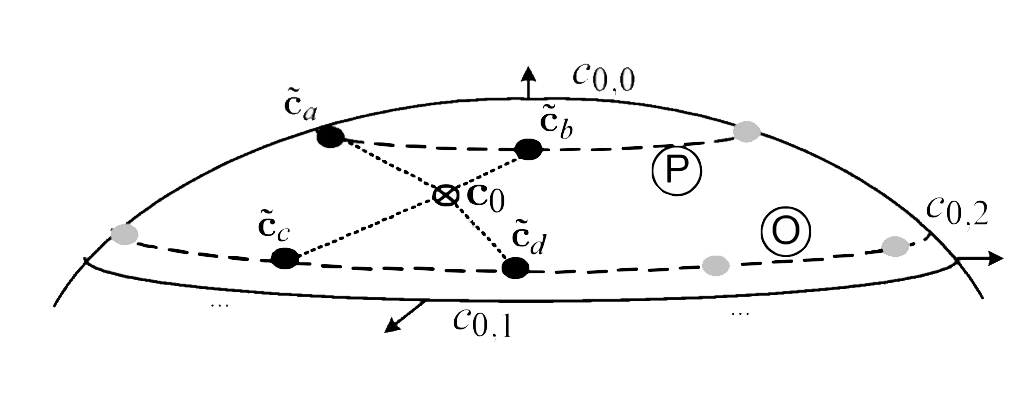
\includegraphics[width=\linewidth]{./img/optim_search_2.png}
  \end{frame}

  % SLIDE : _____________________________________________________________________
  \begin{frame}{Candidate-exclusion}
    \begin{itemize}
      \item Loss in quatization SNR
              %Figure 6: Candidate-exclusion (CE)
      % La exclusion de candidatos se hace en paralelo con la preseleccion. Una vez se han difinido los candidatos a traves de preseleccion se dividen los vecotres en subvectores, y ?????????????????????
    \end{itemize}
  \end{frame}

  % SLIDE : _____________________________________________________________________
  \begin{frame}{Conclusion and results}
    \begin{itemize}
      \item Sample rate 16kHz
      \item Lv = 11
      \item Outperforms G.722
      \item Encoder: 20-25 WMOPS
      \item Decoder: 1-2 WMOPS
      %Comentar los numeros. WMOPS = weighted millions of operations per second. Conclusion: Usando un codebook esferico y procesos eficientes de seleccion se ha conseguido mejorar el CELP tradicional en 0.22MOS 3.83
    \end{itemize}
  \end{frame}


  % SECTION 2:====================================================================

  \begingroup
  \setbeamercolor{section title}{fg=white}
  \setbeamercolor{background canvas}{bg=mDarkTeal}
  \section{Our Implementation}
  \endgroup

  % SLIDE : _____________________________________________________________________
  \begin{frame}{Our Implementation}

  \end{frame}

% ENDING: ======================================================================


\maketitle

\end{document}
